\chapter{Descrição da Abordagem Proposta}
\label{descricao}

Como apresentado na Seção \ref{introducao:objetivos:especificos}, dois dos principais objetivos desta pesquisa são: Propor um modelo baseado em \textit{Redes Bayesianas} para avaliar o TE de equipes ágeis e uma abordagem para utilizar o modelo proposto. Portanto, para utilizar o modelo proposto no Capítulo \ref{modelo}, neste capítulo será descrita a abordagem proposta.

Essa abordagem é dividida em quatro etapas. Propõe-se que essa aborgadem seja utilizada ao final das iterações e antes da reunião de \textit{Retrospectiva da Iteração}. Dessa forma, durante essa reunião, os gerentes de projeto podem reportar os resultados obtidos para a equipe. Além disso, eles podem utilizar esses resultados para auxiliá-los na tomada de decisões para o \textit{Planejamento da Iteração} que acontecerá em seguida. Portanto, neste capítulo, serão descritas todas as etapas dessa abordagem. A Figura \ref{descricao:etapas} contém o fluxo completo da abordagem e as interações entre as etapas.

\begin{figure}[ht!]
\begin{center}
		\fbox{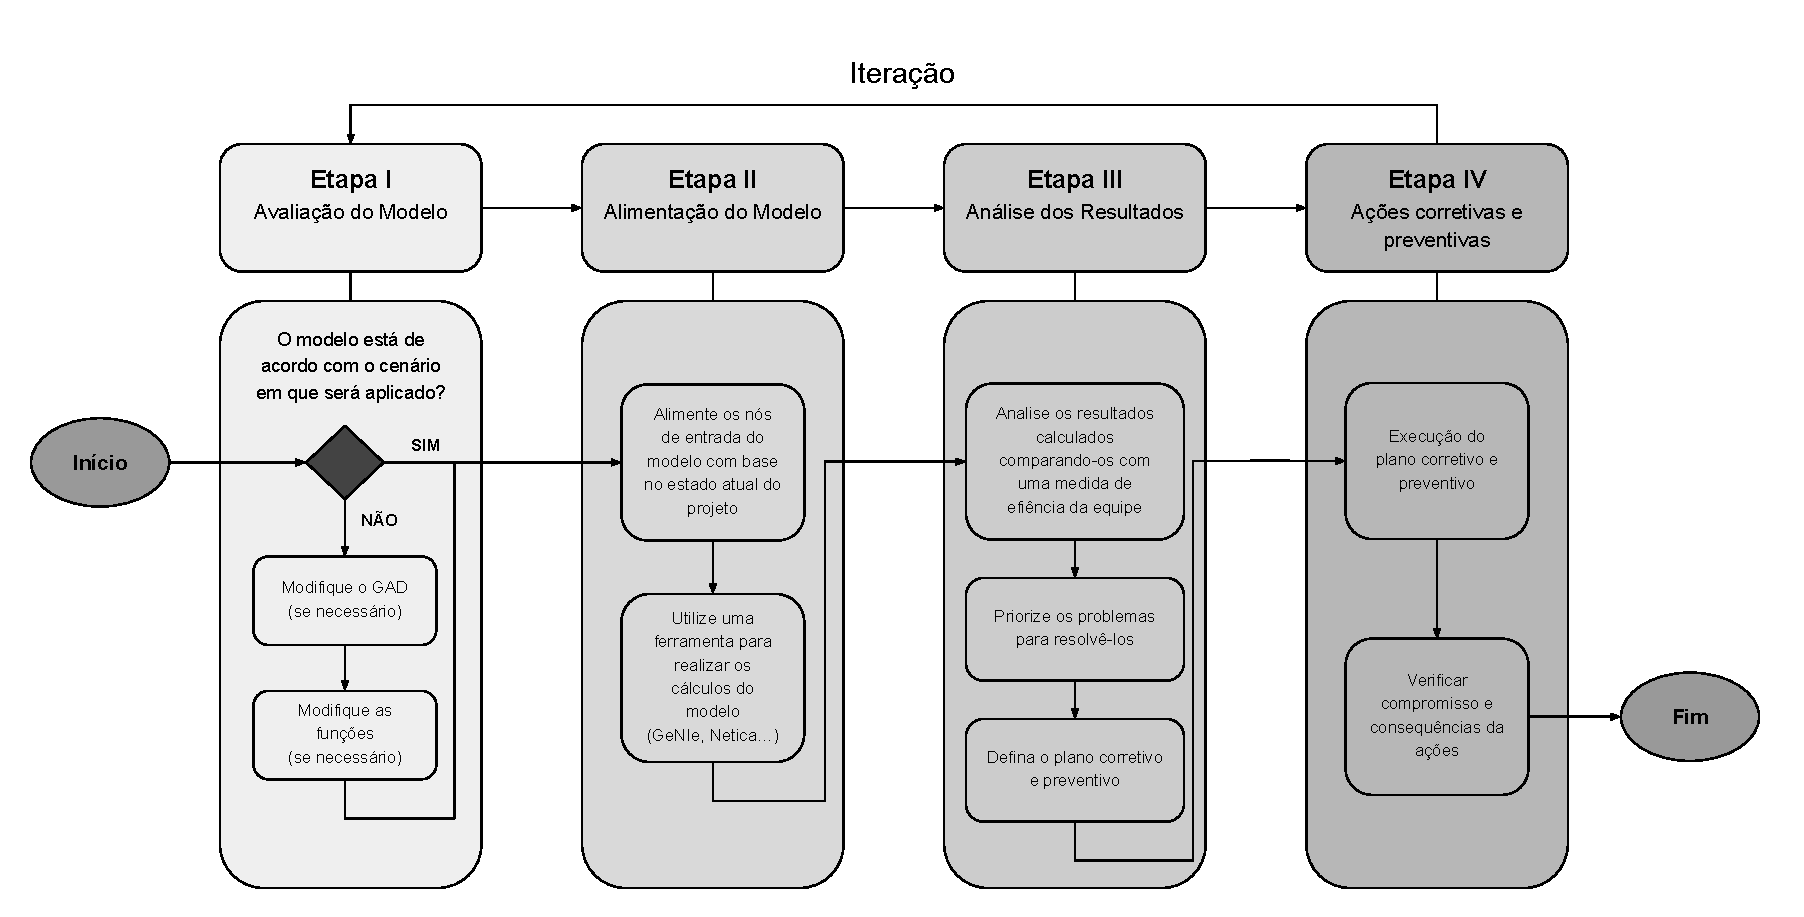
\includegraphics[scale=0.52]{figs/etapasAbordagem.pdf}}
	\end{center}
	\caption{Abordagem para Utilização do Modelo Proposto.}
	\label{descricao:etapas}
\end{figure}

\subsubsection{Etapa I - Avaliação do Modelo}
\label{descricao:avaliacao}

Esta é a etapa inicial da abordagem. Nesta etapa, o indivíduo que deseja utilizar a abordagem deve avaliar se a estrutura do modelo representa fielmente o contexto atual em que ele será aplicado. Por exemplo, se a equipe para a qual o modelo será utilizado não realiza \textit{Reuniões Diárias}, há a necessidade de remover esse nó do GAD. Por outro lado, caso o modelo não contemple algum fator que seja importante naquele contexto, talvez seja importante adicionar um novo nó que represente esse fator ao GAD. Além disso, também podem haver irregularidades nas funções de probabilidade (i.e., a função para um determinado nó deveria ser diferente, ou os pesos de uma função não fazem sentido naquele contexto). Assim, caso julgue necessário, o indivíduo precisará modificar o GAD e/ou as funções de probabilidade para garantir a consistência do modelo em relação ao contexto em que ele está sendo aplicado. Entretanto, caso seja necessário muito esforço para modificar o modelo, talvez seja melhor construir um novo modelo desde o princípio.

O resultado desta etapa deve ser um modelo consistente com o contexto atual do projeto. Portanto, ao final de cada iteração, que é o momento em que essa abordagem deve ser colocada em prática, esta etapa deve ser realizada. Essa periodicidade se deve porque podem haver mudanças no processo e na equipe que venham a contribuir para que o modelo não corresponda ao contexto atual do projeto.

\subsubsection{Etapa II - Alimentação do Modelo}
\label{descricao:alimentacao}

Nesta etapa, o indivíduo precisa alimentar os nós de entrada. Idealmente, seria possível alimentar todos os nós de entrada com evidências. Contudo, como o fator principal abordado neste trabalho e os fatores que o influenciam são subjetivos, a incerteza deve ser a mesma para todos os estados possíveis. Dessa forma, em vez de alimentar os nós de entrada do modelo com dados objetivos, os indivíduos que desejarem utilizar esta abordagem devem indicar, dentre os estados possíveis, um estado para cada um dos nós de entrada. Como forma de facilitar a realização desta etapa, no Apêndice \ref{questionarios} estão definidas perguntas que correspondem aos nós de entrada do modelo. O mapeamento das respostas dessas perguntas para os possíveis estados dos nós entrada também é descrito nesse Apêndice.

Após responder as perguntas e, em seguida, selecionar um estado para cada um dos nós de entrada, os resultados devem ser calculados utilizando uma ferramenta específica de \textit{Redes Bayesianas} (e.g., GeNIe\footnote{\url{http://genie.sis.pitt.edu/}}, Netica\footnote{\url{http://www.norsys.com/}} e AgenaRisk). Os resultados do modelo são dados com probabilidades para cada estado possível de todos os nós do modelo.

\subsubsection{Etapa III - Análise dos Resultados}
\label{descricao:analise}

Após obter os resultados calculados pelo modelo, há a necessidade de analisá-los para detectar possíveis problemas que estão afetando a qualidade do TE. O objetivo desta etapa é avaliar a qualidade do TE na recém-acabada iteração e elaborar um plano de ações corretivas e preventivas para garantir a melhoria contínua do produto final e do processo.

Como o fator principal e os fatores que o influenciam são subjetivos, talvez haja dificuldade em avaliar os resultados. Contudo, a qualidade do TE influencia na eficiência da equipe. Esse fator, por sua vez, depende não apenas da qualidade do TE, mas também do \textit{Planejamento da Iteração}, da complexidade das estórias que precisam ser entregues, dentre outros fatores. Portanto, para facilitar a análise dos dados, propõe-se que os indivíduos que utilizam esta abordagem adotem os resultados calculados pelo modelo como indicadores de uma determinada métrica que represente a eficiência da equipe. Dessa forma, em vez de analisar os resultados calculados comparando-os com resultados esperados pelos gerentes de projeto, a análise será menos sujeita a viés. Entretanto, é necessário atentar para o fato de que o TE não é o único fator que influencia a eficiência da equipe e que todos os outros fatores devem ser levados em consideração . Logo, para realizar a análise dos dados, talvez seja necessário fazer algumas presunções, que podem afetar a validade dessa análise.


\subsubsection{Etapa IV - Ações Corretivas e Preventivas}
\label{descricao:acoes}

Baseado nos resultados calculados pelo modelo e pelas análises realizadas, um plano preventivo e corretivo é elaborado para garantir a melhoria contínua do produto final e do processo, além do TE. Portanto, nesta etapa da abordagem esse plano é executado. Ao final da execução do plano, é necessário verificar o compromisso da equipe em relação às açoes que foram tomadas e quais as suas consequências dessas ações.
